\section{Verdict Generation}\label{sec:verdicts}
The first matching rule applies (Fig.~\ref{fig:verdictflow}): (1) identical sources give no verdict; (2) any confirmed-difference input gives \DIV; (3) any blocking condition gives \INS{} with the lowest-ranked code as primary reason and the others as secondary; (4) otherwise \NDO{} at the highest level whose floors hold. Blocking conditions include import or entry failure; unsupported signature or alignment failure; sandbox failure; unconfirmed or environment-sensitive candidate; unmodelled changed lines; a quarantined input; exactly one side limited; truncated capture; no usable input or unobservable (lossy) outcome; an unactivated changed unit; and an S1 floor failing. The reason-code enumeration is closed (18 codes); several codes are rarely or never produced (ambiguous entry, blind-spot dominance), so the \INS{} vocabulary is partly aspirational.

\begin{figure}[t]\centering
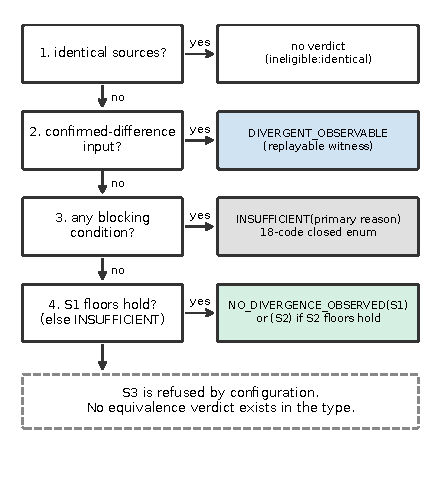
\includegraphics[width=0.92\columnwidth]{../../results/v7b_phase2_summary/figures/fig_p2_verdict_flow.pdf}
\caption{Verdict flow: first match wins; no equivalence verdict exists.}\label{fig:verdictflow}
\end{figure}

Equivalence cannot be emitted because the verdict type asserts a closed value set; this is a naming guarantee. Two rules of the Phase 2 engine matter for the results. First, an equality established on a lossy or degenerate canonical form does not count as the S1 input. Second, changed lines without executable code (for example a continuation line of a multi-line statement) are \texttt{unmodelled\_change}, a conservative blocker (rule A-U1); the rule is unrefined, because continuation lines of an executable statement are not mapped to the statement, and its refinement is an open design decision. A defect found earlier by independent review (a no-run input silently dropped, making \NDO{} reachable with an incomplete input) was fixed before Phase 2.
